
\section{Methodology}

We begin by importing the Sleep-EDF data provided in EDF (European Data Format). The raw EEG recordings are loaded using MNE's \texttt{read\_raw\_edf} function, and corresponding annotations are aligned using \texttt{read\_annotations}. We optionally exclude all non-EEG channels unless explicitly required, focusing on EEG signals for our analysis. The dataset includes two EEG channels: \texttt{Fpz-Cz} and \texttt{Pz-Oz}, which are the primary input sources in our work.

During loading, we crop the signal to reduce unnecessary wake-time data, retaining 30 minutes before the first sleep stage and 30 minutes after the last. This ensures that our training data remains focused around relevant sleep activity. The channel names are cleaned by stripping prefixes for standardization.

After loading and cropping, we segment the data into fixed-length 30-second epochs using the known sampling frequency of the recordings. Only epochs labeled with valid sleep stages — specifically stages W, N1, N2, N3, and REM — are retained. For each epoch, the raw data is extracted and structured into a format suitable for training.

Once all epochs are collected, we flatten the 3D EEG data (epochs $\times$ channels $\times$ time points) into 2D arrays (epochs $\times$ features). This is necessary for traditional machine learning classifiers. To address class imbalance in sleep stages, we apply SMOTE (Synthetic Minority Oversampling Technique) to generate balanced training samples.

The balanced dataset is then split into training and testing sets in an 80-20 ratio. We train a  Machine Learning   on the training data. After training, predictions are made on the test set, and the model is evaluated using standard metrics including classification report and confusion matrix. The confusion matrix is visualized using a heatmap to give a clear view of the stage-wise performance of the classifier.


\section{Dataset Information}

We have used the Sleep-EDF Dataset available at \url{https://www.physionet.org/content/sleep-edfx/1.0.0/}. For our experiments, we selected recordings from approximately 30 patients, resulting in 60 files — 30 EDF (European Data Format) recordings and their corresponding hypnogram annotation files. The EDF files include various bio-signals captured through multiple channels. The hypnogram files contain sleep stage annotations, specifying the start time and type of each stage (Wake, N1, N2, N3, N4, REM) with timestamps in the HH:MM:SS format.

The EDF recordings consist of a range of physiological signals, including EEG (\texttt{Fpz-Cz} and \texttt{Pz-Oz}), EOG, EMG (submental), rectal temperature, and oro-nasal respiration. Each channel provides continuous signal recordings at a specific sampling frequency (Hz), which are used as input features for our downstream machine learning pipeline. From these signals, we derive two essential inputs: spatial features, used to construct graph-based representations, and temporal features, which capture the sequence and timing dynamics necessary for modeling the sleep process.


\begin{figure}
	\centering
	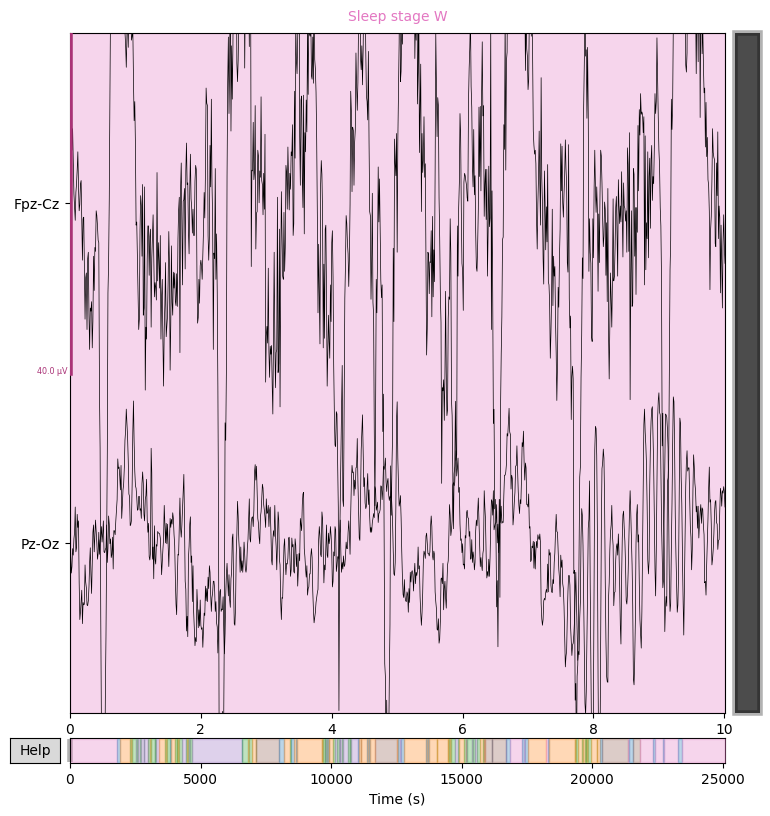
\includegraphics[width=0.4\linewidth]{"./img/paper_1/EEG_Filter_chanel.png"}
	\caption{Filter EEG Chanels}
	\label{fig:eegfilterchanel}
\end{figure}


\section{Preprocessing}

This study applied machine learning techniques to classify sleep stages using EEG signals. The preprocessing pipeline included several crucial steps: channel mapping, data cropping, signal filtering, epoch creation, label mapping, and class balancing using SMOTE. These steps ensured clean, well-structured input for feature extraction and model training. The extracted features spanned time-domain, frequency-domain, and time-frequency representations. Multiple machine learning models—Gradient Boosting, Random Forest, Support Vector Machine (SVC), and Bagging—were trained and evaluated using metrics such as accuracy, precision, recall, and F1-score with cross-validation to assess generalization. The trained models were finally used to classify unseen EEG data into five sleep stages: Wake, N1, N2, N3, and REM.

\paragraph{A. Dataset Acquisition}

EEG signals were recorded using non-invasive electrodes placed on the scalp of human volunteers, capturing brain electrical activity during overnight sleep studies. Additional demographic data such as age, gender, medical history, and sleep habits were collected to provide contextual understanding. The data collection took place in controlled conditions to minimize noise and interference. Manual inspection of the raw EEG was performed to reject or correct artifacts where necessary, ensuring the quality of the input data. The final recordings were saved in standard EDF format for compatibility with downstream analysis. The dataset used in this study was sourced from publicly available Sleep-EDF recordings, which include EEG data and associated hypnogram annotations reflecting sleep stages.

\paragraph{B. Data Preprocessing}

Preprocessing was applied to prepare EEG data for modeling. Channel mapping was done to identify relevant EEG channels, particularly \texttt{Fpz-Cz} and \texttt{Pz-Oz}, and irrelevant or noisy channels were excluded. Data cropping was applied to isolate the sleep period from wake periods based on annotation markers. The signals were then filtered to remove noise and isolate specific frequency bands important for sleep analysis.

Epochs of 30-second duration were created from continuous EEG signals to structure the data for machine learning. Sleep stage labels corresponding to these epochs were derived from hypnogram annotations. Given the naturally imbalanced class distribution in sleep stage data (e.g., fewer REM and N1 stages), the SMOTE algorithm was employed to oversample the minority classes, thereby enhancing model robustness. After preprocessing, the dataset was split into training and testing subsets. This enabled reliable training of models and unbiased performance evaluation. The output from preprocessing was then used in the feature extraction and modeling stages.




\section{Model Architecture and Learning Framework}


The core modeling pipeline begins with transforming the raw EEG data into structured epochs suitable for machine learning classification. Each EEG recording is segmented into 30-second epochs using the sampling frequency and annotated sleep stages. Only valid sleep stages (Wake, N1, N2, N3, and REM) are retained for downstream processing. After epoching, each segment is extracted using the \texttt{mne.Epochs} function, resulting in structured EEG data with consistent time windows. These segments are then reshaped into two-dimensional feature vectors where each row corresponds to an epoch and each column to a time-series sample across all EEG channels.

To address the class imbalance inherent in sleep stage data, the SMOTE (Synthetic Minority Over-sampling Technique) algorithm is applied. This balances the dataset by synthetically generating new examples in underrepresented classes. The balanced dataset is then split into training and testing sets in an 80:20 ratio.  

\begin{figure}
	\centering
	\includegraphics[width=0.7\linewidth]{"img/paper_1/Architechture1"}
	\caption{Architecture of Machine Learning Classifiers for Sleep Stage
		Classificatio}
	\label{fig:architechture1}
\end{figure}







\subsection{Random Forest Classifier}

We implemented a Random Forest classifier to establish a strong baseline model for sleep stage classification. The raw EEG recordings were segmented into 30-second epochs, and features were extracted by flattening the multidimensional epoch data. To handle class imbalance, the SMOTE algorithm was applied prior to training. The model was initialized with \textbf{100 decision trees} (\texttt{n\_estimators=100}) and a fixed \textbf{random seed} (\texttt{random\_state=42}) to ensure reproducibility. This configuration allowed the model to generalize well while maintaining robust performance across varying sleep stages.

\subsection{Gradient Boosting Classifier with PCA}

To improve computational efficiency and potentially boost model accuracy, we introduced Principal Component Analysis (PCA), retaining \textbf{95\% of the explained variance} (\texttt{n\_components=0.95}). The reduced feature set was passed to a \textbf{Gradient Boosting classifier} configured with \textbf{30 estimators} (\texttt{n\_estimators=30}), a \textbf{maximum tree depth of 3} (\texttt{max\_depth=3}), and a \textbf{learning rate of 0.1}. Class balancing was again addressed with SMOTE. The same 80-20 train-test split was maintained with \texttt{random\_state=42}. This model leverages the sequential learning of weak classifiers to optimize classification performance over multiple iterations.

\subsection{Ensemble Learning (Voting Classifier)}

\begin{sloppypar}
	For further enhancement, we employed a soft voting ensemble that combines multiple classifiers, each with complementary strengths. The ensemble includes a \textbf{Gradient Boosting Classifier} (\texttt{n\_estimators=50}, \texttt{max\_depth=3}, \texttt{learning\_rate=0.1}), a \textbf{Random Forest Classifier} (\texttt{n\_estimators=50}, \texttt{max\_depth=3}), a \textbf{Support Vector Classifier (SVC)} with an RBF kernel and probability estimates enabled, and a \textbf{Bagging Classifier} (\texttt{n\_estimators=30}, \texttt{max\_samples=1.0}, \texttt{max\_features=1.0}). These classifiers were integrated using a \textbf{soft voting strategy} in the \texttt{VotingClassifier(voting='soft')} to average their probabilistic predictions.
	
	Feature reduction was again performed using PCA with 95\% variance retention. This ensemble approach leverages model diversity to achieve improved generalization and more stable predictions across sleep classes.
\end{sloppypar}


\section{Results and Evaluation}

This section presents the results and evaluations for the models trained, including Random Forest, Bagging, Ensemble Learning, and Gradient Boosting. The following figures summarize the performance metrics for each model.

\subsection{Random Forest}

For the Random Forest model, we present the following evaluation metrics:

\begin{figure}[H]
	\centering
	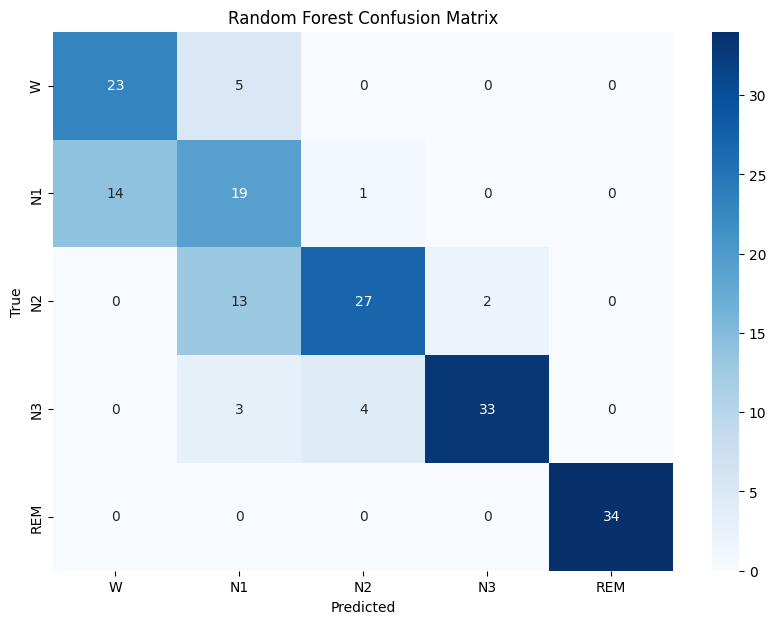
\includegraphics[width=\textwidth]{img/paper_1/random_forest_confusion_matrix.png}
	\caption{Random Forest Confusion Matrix}
\end{figure}

\begin{figure}[H]
	\centering
	\includegraphics[width=\textwidth]{img/paper_1/accuracy_curve.png}
	\caption{Random Forest Accuracy Curve}
\end{figure}

\begin{figure}[H]
	\centering
	\includegraphics[width=\textwidth]{img/paper_1/loss_curve.png}
	\caption{Random Forest Loss Curve}
\end{figure}

\begin{figure}[H]
	\centering
	\includegraphics[width=\textwidth]{img/paper_1/precision_per_class.png}
	\caption{Random Forest Precision Per Class}
\end{figure}

\subsection{Bagging Classifier}

For the Bagging Classifier model, we present the following evaluation metrics:

\begin{figure}[H]
	\centering
	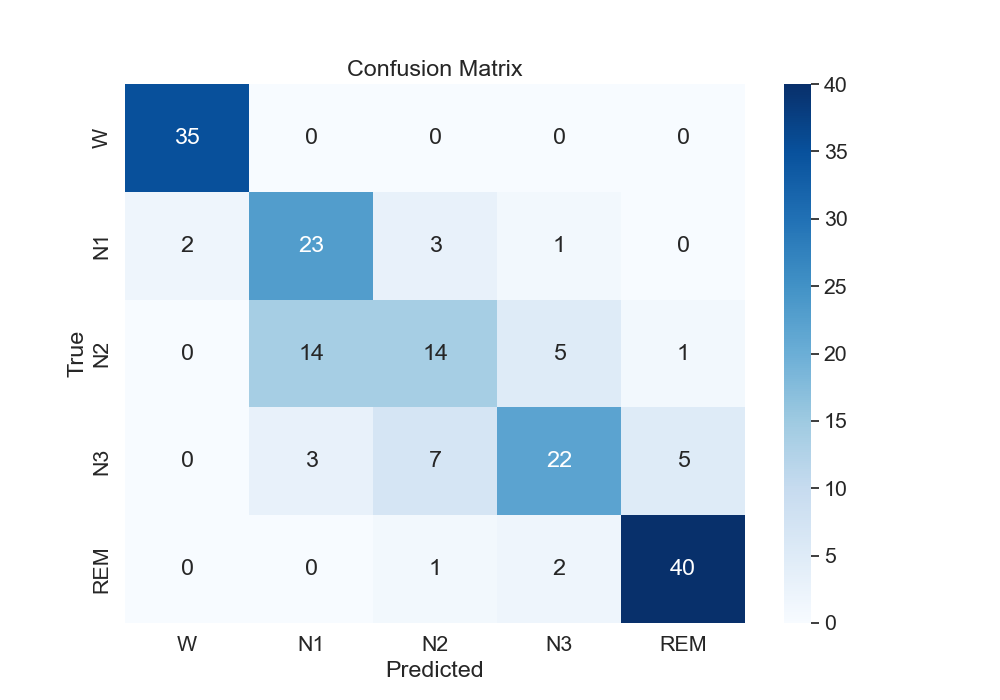
\includegraphics[width=\textwidth]{img/paper_1/BG_confusion_matrix.png}
	\caption{Bagging Classifier Confusion Matrix}
\end{figure}

\begin{figure}[H]
	\centering
	\includegraphics[width=\textwidth]{img/paper_1/accuracy_curve.png}
	\caption{Bagging Classifier Accuracy Curve}
\end{figure}

\begin{figure}[H]
	\centering
	\includegraphics[width=\textwidth]{img/paper_1/loss_curve.png}
	\caption{Bagging Classifier Loss Curve}
\end{figure}

\begin{figure}[H]
	\centering
	\includegraphics[width=\textwidth]{img/paper_1/precision_per_class.png}
	\caption{Bagging Classifier Precision Per Class}
\end{figure}

\subsection{Ensemble Learning}

For the Ensemble Learning model, we present the following evaluation metrics:

\begin{figure}[H]
	\centering
	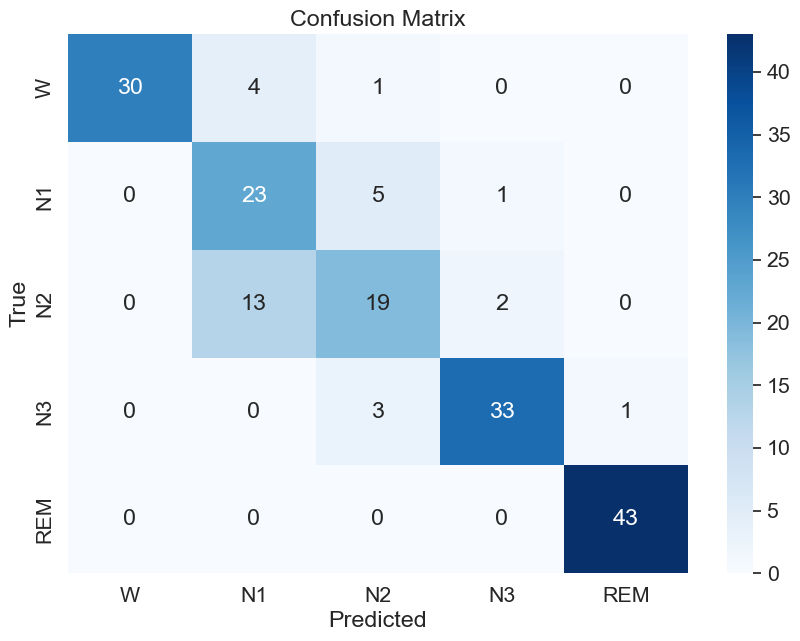
\includegraphics[width=\textwidth]{img/paper_1//Ensemble_confusion_matrix.png}
	\caption{Ensemble Learning Confusion Matrix}
\end{figure}

\begin{figure}[H]
	\centering
	\includegraphics[width=\textwidth]{img/paper_1//accuracy_curve.png}
	\caption{Ensemble Learning Accuracy Curve}
\end{figure}

\begin{figure}[H]
	\centering
	\includegraphics[width=\textwidth]{img/paper_1//loss_curve.png}
	\caption{Ensemble Learning Loss Curve}
\end{figure}

\begin{figure}[H]
	\centering
	\includegraphics[width=\textwidth]{img/paper_1//precision_per_class.png}
	\caption{Ensemble Learning Precision Per Class}
\end{figure}

\subsection{Gradient Boosting}

For the Gradient Boosting model, we present the following evaluation metrics:

\begin{figure}[H]
	\centering
	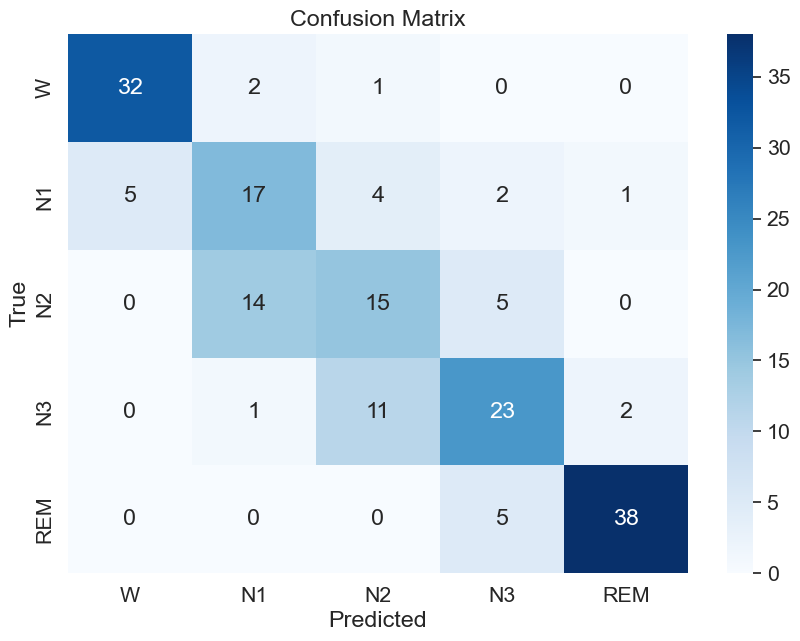
\includegraphics[width=\textwidth]{img/paper_1//confusion_matrix.png}
	\caption{Gradient Boosting Confusion Matrix}
\end{figure}

\begin{figure}[H]
	\centering
	\includegraphics[width=\textwidth]{img/paper_1//accuracy_curve.png}
	\caption{Gradient Boosting Accuracy Curve}
\end{figure}

\begin{figure}[H]
	\centering
	\includegraphics[width=\textwidth]{img/paper_1//loss_curve.png}
	\caption{Gradient Boosting Loss Curve}
\end{figure}

\begin{figure}[H]
	\centering
	\includegraphics[width=\textwidth]{img/paper_1//precision_per_class.png}
	\caption{Gradient Boosting Precision Per Class}
\end{figure}
